\chapter{Графи}
\index{граф}
\label{chap:graph}


\begin{dfn}
  Неориентиран граф\index{неориентиран!граф} $G$ е наредена тройка $(V,E,\psi_G)$, където
  $V$ е непразно множество, $V,E$ са непресичащи се множества, и $\psi_G$ асоциира с всеки елемент $e\in E$
  ненаредена двойка от елементи на $V$.
  Елементите на $V$ наричаме върхове, а елементите на $E$ ребра.
\end{dfn}

Нека да въведем някои означения.
Под прост граф\index{прост!граф} $G$ ще разбираме неориентиран граф без примки и повтарящи се ребра.
С $\delta(G)$\index{$\delta(G)$} ще означаваме минималната степен в графа $G$, а с $\Delta(G)$\index{$\Delta(G)$} - максималната.
Означаваме $\nu(G) = |V|, \epsilon(G) = |E|$.
Броят на свързаните компоненти на $G$ означаваме с $\omega(G)$.

\begin{problem}
  Докажете, че $\delta \leq \frac{2\varepsilon}{\nu} \leq \Delta$.
\end{problem}
\begin{proof}
  $\nu\delta \leq\sum_{1\leq i \leq\nu} deg_G(v_i) \leq \nu\Delta$.
\end{proof}

\begin{problem}
  Нека $G$ е свързан граф.
  Докажете, че всеки два най-дълги пътя в свързан граф имат общ връх.
\end{problem}
\begin{proof}
  Да разгледаме два най-дълги пътя в $G$, $\pi_1 = [u_1,\dots,u_n]$ и $\pi_2 = [v_1,\dots,v_n]$ и да допуснем, че $\pi_1$ и $\pi_2$
  нямат общи върхове.
  $G$ е свързан, следователно има път $\rho$ от $u_i$ до $v_j$, за някои $i,j$.
  Със сигурност по $\rho$ има ребро, което не участва нито в $\pi_1$, нито в $\pi_2$, защото иначе ще имаме общ връх между $\pi_1$ и $\pi_2$.
  Но така пък имаме път с дължина поне $n+1$, което е противоречие.
\end{proof}

\begin{problem}%GTWA 1.6.13
  Покажете, че ако $G$ е прост, $diam(G) = 2$ и $\Delta = \nu - 2$, то $\varepsilon \geq 2\nu - 4$.
\end{problem}

\begin{lemma}[Денеш Кьониг]\index{Кьониг, Денеш!теорема}
  Ако $G$ е свързан граф с безкрайно много върхове и всеки връх има крайна степен, то всеки връх в $G$ е част от 
  безкрайно дълъг прост път (т.е. път без повтарящи се върхове).
\end{lemma}


\section{Дървета}
\label{sect:tree}

\begin{dfn}
  Дърво е свързан граф без цикли.
\end{dfn}

\begin{thm}
  В дърво, между всеки два върха има единствен път.
\end{thm}

\begin{thm}
  Ако $G$ е дърво, то $\epsilon = \nu - 1$.
\end{thm}
\begin{proof}
  С индукция по $\nu$. За $\nu = 1$ е ясно.
  Да допуснем за $G$ с брой ребра $<\nu$ и ще докажем за $G$.
  Нека $uv\in E$ и $G'$ се получава като изтрием това ребро.
  Получаваме два свързани ациклични графа $G_1, G_2$.
  Следователно те са дървета и от и.п. 
  \[\varepsilon(G_1) = \nu(G_1) - 1\ \&\ \varepsilon(G_2) = \nu(G_2) - 1.\]
  Получаваме, че 
  \[\varepsilon(G - uv) = \varepsilon(G_1) + \varepsilon(G_2) = \nu(G_1) + \nu(G_2) - 2.\]
  Накрая, $\varepsilon(G) = \varepsilon(G-uv) + 1 = \nu(G_1) + \nu(G_2) - 2 + 1= \nu(G) - 1$.
\end{proof}

\begin{corollary}
  Всяко нетривиално дърво има поне два върха със степен 1.
\end{corollary}
\begin{proof}
  Ясно е, че $(\forall v\in V)[d(v) \geq 1]$.
  Знаем, че $\Sigma_{v\in V}d(v) = 2\varepsilon = 2\nu - 2$, от където следва, че има поне два върха със степен 1.
\end{proof}



Означаваме с $\tau(G)$ броят на покриващите дървета на $G$ (не неизоморфните, а всички).

Нека $u\neq v, e = (u,v)\in E$. С $G.e = (E',V')$ означаваме графа получен от $G$, като премахваме реброто $e$ и 
съединяваме краищата $u,v$. Ясно е, че $\nu(G.e) = \nu(G) - 1, \varepsilon(G.e) = \varepsilon(G) - 1, \omega(G.e) = \omega(G)$.

\begin{thm}
  Ако $e\in E$ не е примка, то
  $\tau(G) = \tau(G-e) + \tau(G.e)$.
\end{thm}
\begin{proof}
  $\tau(G) = n + m$, където $n$ е броят на покриващите дървета на $G$, в които не участва $e$
  и $m$ е броят на покриващите дървета, в които участва $e$.
  Ясно е, че $n = \tau(G-e)$.
  На всяко покриващо дърво $T$, в което участва $e$, съответства покриващо дърво $T.e$ на $G.e$.
  Това съответствие е взаимно-еднозначно, следователно $m = \tau(G.e)$.
\end{proof}

\begin{problem}
  Колко на брой са всички изоморфни и неизоморфни покриващи дървета на $K_3,K_4$ ?
\end{problem}

\begin{thm}[Кейли]\index{Кейли} %GTWA , page 35
  $\tau(K_n) = n^{n-2}$.
\end{thm}
\begin{proof}[Pr\"ufer, 1918]
  Нека да означим с $N = \{1,2,\dots,n\}$ ребрата на $K_n$.
  Обърнете внимание, че $n^{n-2}$ е броят на думи с дължина $n-2$ над азбуката $N$.
  Искаме да построим биекция между множеството от всички покриващи дървета на $K_n$ 
  и множеството от всички такива думи. За целта ще считаме, че върховете на дърветата
  са номерирани с числата от $1$ до $N$.

  Да разгледаме едно дърво $T$ от $K_n$. Ще асоциираме с него редица от числа $(t_1,t_2,\dots,t_{n-2})$.
  Нека $s_1$ да дъде първия връх със степен $1$ и $t_1$ да бъде неговия съсед.
  Нека $s_2$ да бъде първия връх със степен $1$ в $T - s_1$ и $t_2$ да бъде неговия съсед.
  Продължаваме тази процедура докато намерим $t_{n-2}$ и в дървото са останали само два върха.

  Лесно се доказва, че с тази процедура получаваме различни думи за различни покриващи дървета на $K_n$.
  
  Остава да видим как от една такава дума можем да възтановим покриващото дърво $T$.
  Първо, обърнете внимание, че всеки връх участва $t$ $d_T(t) - 1$ пъти в $(t_1,\dots,t_{n-2})$.
  Това означава, че върховете със степен $1$ са точно тези върхове, които не са измежду $t_1,\dots, t_{n-2}$.
  Нека $s_1$ да бъде първия връх от $N$, който не е в $(t_1,\dots,t_{n-2})$. Тогава свързваме $s_1$ с $t_1$.
  Продължаваме с първия връх $s_2$ от $N\setminus\{s_1\}$, който не е в $(t_2,\dots,t_{n-2})$.
  Свързваме $s_2$ с $t_2$. 
  Продължавайки по този начин, формираме $n-2$ ребра $(s_1,t_1), \dots, (s_{n-2},t_{n-2})$.
  Получаваме дървото като добавим ребро между останалите два върха.

  Отново лесно се проверява, че от различни думи се получават различни покриващи дървета.
\end{proof}

\begin{remark}
  Обърнете внимание, че $n^{n-2}$ {\em не} е броят на всички неизоморфни покриващи дървета на $K_n$, а
  а броят на различните покриващи дървета. Например, броят на неизоморфните покриващи дървета на $K_6$
  са 6.
\end{remark}

\begin{corollary}
  Нека $d_1,\dots, d_n$ са положителни цели числа и $\sum_i d_i = 2n - 2$.
  Тогава съществуват точно $\frac{(n-2)!}{\prod(d_i - 1)!}$ дървета с върхове $\{1,\dots,n\}$, 
  като всеки връх $i$ има степен $d_i$.
\end{corollary}
\begin{proof}
  В едно дърво сумата от степените на върховете е точно $2n - 2$.
  Всеки връх $x$ се появява $d_T(x) - 1$ пъти в кода на Прюфер.
\end{proof}



\begin{problem}
  \begin{enumerate}[1)]
  \item
    Докажете, че ако $e\in E(G)$ и $e$ не е примка, то
    $\tau(G) = \tau(G - e) + \tau(G\cdot e)$.
  \item
    Покажете, че ако $e$ е ребро в $K_n$, то $\tau(K_n - e) = (n-2)n^{n-3}$.
  \end{enumerate}
\end{problem}
\begin{proof}
  \begin{enumerate}[1)]
  \item
    
  \item
    Ще използваме $1)$.
    Тъй като $\tau(K_n - e) = \tau(K_n) - \tau(K_n\cdot e)$, то достатъчно е да докажем, че
    $\tau(K_n\cdot e) = 2.n^{n-3}$, защото вече знаем, че $\tau(K_n) = n^{n-2}$.
    Разглеждаме $e$ като връх в графа $K_n\cdot e$.
    $deg_{K_n\cdot e}(e) = 2(n-2)$.
    Нека $G$ да бъде $K_n\cdot e$, но без повтарящи се ребра.
    Тогава $G = K_{n-1}$.
    Тогава $deg_G(e) = n-2$ и следователно върхът $e$ може да очаства
    $n-3$ пъти в кода на Прюфер за $G$.
    Едно покриващо дърво еднозначно се определя от код на Прюфер с дължина $n-3$.
    Ако $e$ е листо в $K_n\cdot e$, то имаме $2.(n-2)^{n-3}$ такива покриващи дървета.
    Ако $e$ се среща веднъж в кода на Прюфер, то $e$ има степен $2$ в покриващото дърво
    и така получаваме
    $\binom{n-3}{1}(n-2)^{n-4}2^2$ на брой покриващи дървета.
    Накрая използваме равенството
    \[n^{n-3} = \sum^{n-3}_{i=0}\binom{n-3}{i}2^i(n-2)^{n-3-i}.\]
\end{enumerate}

\end{proof}


\begin{problem}
  Покажете, че ако $G$ е дърво с $\delta \geq k$, то $G$ има поне $k$ върха със степен 1.
\end{problem}

\begin{problem}
  Нека $G$ да бъде граф с $\varepsilon = \nu - 1$. Покажете, че следните твърдения са еквивалентни:
  \begin{enumerate}
  \item
    $G$ е свързан;
  \item
    $G$ е без цикли;
  \item
    $G$ е дърво.
\end{enumerate}
\end{problem}
\begin{proof}
  С индукция по броя на ребрата, като използваме факта, че щом $\varepsilon = \nu - 1$, то има
  връх със степен 1.
\end{proof}



\section{Основни свойства на графите. Изоморфни графи}
\begin{dfn}
  \begin{enumerate}
  \item
    $n$-клика;
  \item
    Път с дължина $n$;\index{път!граф}
  \item
    цикъл на $n$ върха.\index{цикъл!граф}
\end{enumerate}
\end{dfn}

Броят на ребрата в един граф се нарича размер.
В граф с $n$ върха, максималния размер е $\binom{n}{2}$.

Казваме, че два графа $G$ и $H$ са изоморфни, пишем $G\cong H$, ако
\item съществуват биекции $\theta:V(G)\to V(H)$ и $\phi:E(G)\to E(H)$, като е изпълнено
$(u,v) = e \in E(G) \iff (\theta(u),\theta(v)) = \phi(e) \in E(H)$.
Двойката $(\theta,\phi)$ ще наричаме изоморфизъм между $G$ и $H$.



\begin{problem}
  Нека $D=(V,T)$ е подграф на свързания граф $G=(V,E)$.
  Докажете, че следните условия са еквивалентни:
  \begin{enumerate}
  \item
    $D$ е покриващо дърво на $G$;
  \item
    $|T| = |V|-1$ и $D$ не съдържа цикли;
  \item
    за всеки два върха $u,v\in V$ съществува в $D$ точно един път от $u$ до $v$;
  \item
    $|T| = |V|-1$ и за всяка двойка върхове $u,v\in V$ съществува в $D$ поне един път от $u$ до $v$.
  \item
    $|T| = |V|-1$ и за всяка двойка върхове $u,v\in V$ съществува в $D$ не повече от един път от $u$ до $v$.
  \end{enumerate}
\end{problem}

\begin{dfn}
  \begin{enumerate}
  \item
    Краен неориентиран граф, всички върхове на който са от една и съща степен $d$ се нарича регулярен със степен $d$.  
  \item
    Един граф е свързан, ако между всеки два възела на графа има път.
  \item
    Един граф е двуделен, ако върховете му могат да се разделят на две множества и всяко ребро в графа има по един връх от двете множества.
\end{enumerate}
\end{dfn}


\begin{problem}
  За $G$ прост граф, докажете, че $\varepsilon = \binom{\nu}{2}$ т.с.т.к. $G$ е пълен.
\end{problem}
\begin{proof}
  С индукция по $\nu$.
  $\binom{\nu+1}{2} = \sum^2_{i=0}\binom{\nu}{i}\binom{1}{2-i} = \nu + \binom{\nu}{2}$.
  Ако $\epsilon^\prime =\nu + \binom{\nu}{2}$, то е ясно, че $G^\prime$ е пълен.
  Ако $G^\prime$ е пълен, то е ясно, че $\epsilon^\prime = \nu + \binom{\nu}{2}$.
\end{proof}


\begin{problem}
  Докажете, че в прост граф с $\nu\geq 2$, има поне два върха с еднаква степен.
\end{problem}
\begin{proof}
  Да допуснем, че $d_G(v_i)\neq d_G(v_j)$, за $i\neq j$.
  Тогава имаме връх със степен $\geq \nu$. Това е противоречие с условието, че графът е прост.
\end{proof}

\begin{problem}
  Колко графа с $n$ върха и $m$ ребра има, за които:
  \begin{enumerate}[a)]
  \item
    ненасочени, прости и без повтарящи се ребра;
  \item
    ненасочени и прости;
  \item
    ненасочени, но не непременно прости;
  \item
    насочени и прости и без повтарящи се ребра;
  \item
    насочени и прости;
  \item
    насочени, но не непременно прости.
\end{enumerate}
\end{problem}
\begin{proof}
  \begin{enumerate}[a)]
  \item
    $\binom{\binom{n}{2}}{m}$
  \item
    $\binom{m+\binom{n}{2}-1}{m}$
  \item
    $\binom{m+\binom{n}{2}+n-1}{m}$
  \item
    $\binom{n(n-1)}{m}$
  \item
    $\binom{m+n(n-1)-1}{m}$
  \item
    $\binom{m+n^2-1}{m}$.
  \end{enumerate}
\end{proof}

\begin{problem}
  Докажете, че:
  \begin{enumerate}
  \item
    във всеки неориентиран граф броят на върховете с нечетна степен е четен;
  \item
    всеки регулярен граф с нечетна степен има четен брой върхове;
  \item
    всеки прост граф с $\varepsilon > \binom{\nu-1}{2}$ е свързан;
  \item
    във граф всички върхове имат степен поне $d$.
    Докажете, че в графа има път с дължина $d$.
  \end{enumerate}
\end{problem}
\begin{proof}
  \begin{enumerate}
  \item
    Лесно, като се използва, че $\sum_{v\in V} deg_G(v) = 2\varepsilon$ е четно.
  \item
    Пак лесно.
  \item
    Задачата се решава с индукция по броят на върховете.
    Да допуснем, че твърдението е вярно за всички графи $G$ с $\nu(G)\leq n$.
    Да вземем граф $G(V,E)$ с $\nu(G) = n+1$ и $\varepsilon>\binom{\nu-1}{2}$ и да допуснем, че 
    $G$ не е свързан. Това означава, че има върхове $v_i,v_j\in V$, между които няма път.
    Да вземем произволен връх $p\in V$, различен от $v_i,v_j$.
    Ясно е, че $d_G(p) \leq \nu-2 = n-1$, защото $(p,v_j)\not\in E$ или $(p,v_i)\not\in E$ и няма примки.
    Да разгледаме графа $G^\prime(V^\prime,E^\prime)$, където $V' = V\backslash{\{p\}}$ и 
    $E^\prime$ се получава от $E$ като махнем всички ребра с един край $p$.
    Тогава \[\varepsilon^\prime \geq \varepsilon - (n-1) > \frac{n(n-1)}{2} - (n-1) = \frac{(n-1)(n-2)}{2}.\]
    От индукционното предположение, $G^\prime$ е свързан граф, но $v_i,v_j\in V'$ и между тях няма път.
    Така достигаме до противоречие.
  \item
    Разгледайте най-дългия път $\pi$ в графа.
    Той има дължина $p$. Последния връх в $\pi$ има степен $\geq d$ и всички върхове, с които е свързан 
    са в $\pi$, защото иначе ще можем да образуваме по-дълъг път.
    Следователно, $p \leq d+1$ и следователно съществува път с дължина $d$.
  \end{enumerate}
\end{proof}

\begin{remark}
  Ако за графът $G$ е изпълнено \[\binom{\nu-1}{2} < \varepsilon \leq \binom{\nu}{2},\]
  то той със сигурност е свързан.
\end{remark}

\begin{problem}
  \begin{enumerate}
  \item
    Докажете, че има 11 неизоморфни прости графа с 4 върха.
  \item
    Намерете броя на ребрата на граф без цикли с $n$ върха и $k$ компоненти.
  \item
    Докажете, че при $n>0$, $n$-мерния двоичен куб е свързан двуделен граф, има $2^k$ върхове и $k2^{k-1}$ ребра.
\end{enumerate}

\end{problem}
\begin{proof}
  \begin{enumerate}
  \item
    
  \item
    $n-k-1$.
  \item
    За двуделен - едната компонента е от тези върхове с четен брой единици, другата с нечетен.
\end{enumerate}

\end{proof}


\begin{thm}[Денеш Кьониг]\index{Кьониг, Денеш!теорема}
  Във всеки двуделен граф, броят на ребрата в максимално съчетание е равен на броя на ребрата в минимално покритие на върховете. 
\end{thm}



\begin{problem}
  Дадено е множество от различни върхове $V=\{v_1,\dots,v_n\}$.
  Колко ориентирани графа могат да се съставят от $V$, като има най-много едно ребро между всяка двойка върхове $v_i,v_j\in V$.
  (Считаме, че два изоморфни графа са различни.)
\end{problem}
\begin{proof}
  За всяка двойка $v_i,v_j\in V$ имаме един от трите случая - $v_i$ и $v_j$ не са свързани, 
  имаме ребро $(v_i,v_j)$ или имаме ребро $(v_j,v_i)$.
  Имаме $\binom{n}{2}$ двойки върхове, следователно отговорът е $3^{\binom{n}{2}}$.
\end{proof}

\begin{dfn}
  Даден е {\bf свързан граф} $G=(V,E)$.
  Разстоянието $dist_G(u,v)$ е дефинирано като най-късия път между $u$ и $v$. (не е за цикъл, т.е. $u\neq v$).
  Ако няма път между $u$ и $v$ в $G$, то $dist_G(u,v) = \infty$.
  Диаметърът\index{диаметър!граф} $diam(G)$ на $G$ е дефиниран като най-голямото разстояние между върхове в $G$, т.е.
  $diam(G) = max_{u,v\in V}dist_G(u,v)$.
  Ексцентричност $ecc(v) = max_{u\in V}dist_G(u,v)$.
  Радиус\index{радиус!граф} $rad(G) = min_{v\in V}ecc(v)$.
\end{dfn}


\begin{problem}
  За произволни върхове $u,v,w$ в графа $G$, 
  $dist(u,v)+dist(v,w) \geq dist(u,w)$
\end{problem}


\begin{problem}
  Нека $G = (V,E)$ е свързан граф. Докажете, че:
  \begin{enumerate}
  \item
    Нека добавим нов връх към $V$ и произволни ребра към $E$ за да получим нов свързан граф $G^\prime$.
    Докажете, че $diam(G)\geq diam(G^\prime)$;
  \item
    Нека $V' = V\setminus{\{u\}}$ за $u\in V$ и $G' = (V',E')$ остава да бъде свързан.
    Докажете, че $diam(G')\geq diam(G)$;
  \item
    $rad(G)\leq diam(G)\leq 2rad(G)$;
  \item
    За всяко $n\in \mathbb{N}^+$, съществуват свързани графи $G_1$ и $G_2$ с
    $diam(G_1)=diam(G_1)=n$ и $diam(G_2) = 2rad(G_2) = 2n$.
\end{enumerate}
\end{problem}
\begin{proof}
  \begin{enumerate}
  \item
    ясно.
  \item
    ясно.
  \item
    Очевидно, $rad(G)\leq diam(G)$.\\
    Сега, нека $d_1,d_2$ са върховете в $G$ с най-голямо $d_G(d_1,d_2)$.
    Нека $v'$ да бъде този връх, за който $ecc(v') = rad(G)$.
    \[diam(G)\leq d_G(v',d_1) + d_G(v',d_2).\]
    \[d_G(v',d_1) + d_G(v',d_2) \leq ecc(v') + ecc(v') = 2rad(G).\]
    \[diam(G)\leq 2rad(G).\]
  \item
    Взимаме цикъл с $2n$ върха.
    Взимаме линеен граф с $2n+1$ върха .
\end{enumerate}

\end{proof} 


\begin{problem} % зад. 1.19 от Глава VI, Графьи и Сеть
  Нека $G$ е произволен граф без примки и кратни ребра, а $\overline{G}$ е неговото допълнение. Докажете, че:
  \begin{enumerate}
  \item
    поне един от графите $G$, $\overline{G}$ е свързан;
  \item
    ако в $G$ има повече от 4 върха, то поне в един от графите $G$, $\overline{G}$ има цикъл;
  \item
    ако $G$ е или несвързан или $diam(G)\geq 3$, то $\overline{G}$ е свързан и $diam(\overline{G})\leq 3$;
  \item
    ако $v$ - разделящ връх в $G$, то той не се явява разделящ в $\overline{G}$.
\end{enumerate}
\end{problem}

\begin{proof}
  \begin{enumerate}
  \item
    С индукция по броя на върховете.
    Нека $\nu = n + 1$. Да разгледаме $G$ и $\overline{G}$.
    Да разгледаме $V^\prime = V - \{u\}$, за $u$ произволен връх от $V$.
    Без ограничение на общността, нека $G^\prime$ е свързан.
    Ако $u$ е край на поне едно ребро от $E$, то очевидно $G$ е свързан.
    Ако $u$ не е край на нито едно ребро от $E$, то очевидно $\overline{G}$ е свързан.
  \item
    лесно.
  \item
    Първо, нека да разгледаме $G$ несвързан.
    Тогава съществуват $u,v\in V$, между които няма път.
    Тогава знаем, че $\overline{G}$ е свързан и $(u,v)\in\overline{E}$.
    $A = \{a\in V\mid\pi_{\overline{G}}(u,a)\}$ и $B = \{b\in V\mid\pi_{\overline{G}}(v,b)\}$.
    Ясно е, че $A\cup B = V$, защото $(u,v)\not\in E$.
    За да докажем, че $diam(\overline{G})\leq 3$ е необходимо да разгледаме случаите:
    \begin{enumerate}[a)]
    \item
      Нека да вземем $a,b\in A$.
      Най-краткият път между тях в $\overline{G}$ е $a,u,b$.
    \item
      Нека да вземем $a,b\in B$.
      Най-краткият път между тях в $\overline{G}$ е $a,v,b$.
    \item
      Нека да вземем $a\in A,b\in B$.
      Най-краткият път между тях в $\overline{G}$ е $a,u,v,b$.
    \end{enumerate}
    
    Нека сега $G$ е свързан и $diam(G)\geq 3$.
    Имаме, че $\overline{G}$ също е свързан, защото иначе ще имаме противоречие с $diam(G)\geq 3$.
    Това означава, че има смисъл да говорим за $diam(\overline{G})$.
    Нека да махнем един връх от $G$ и да получим $G^\prime$
    Ако $G^\prime$ е несвързан, тогава $\overline{G^\prime}$ е свързан и от индукционното предположение, $diam(\overline{G^\prime})\leq 3$.
    Като добавим $u$, имаме, че $diam(\overline{G})\leq diam(\overline{G^\prime})\leq 3$.
    Ако $G^\prime$ е свързан, то $diam(G^\prime)\geq diam(G)\geq 3$, тогава от и.п. $diam(\overline{G'})\leq 3$ (тук също знаем, че $\overline{G'}$ е свързан). Тогава като добавим $u$ получаваме отново, че $diam(\overline{G})\leq diam(\overline{G^\prime})\leq 3$.
  \item
\end{enumerate}

\end{proof}


\begin{problem} % зад 1.20
  Граф (без примки и кратни ребра) $G$ се нарича самодопълнителен, ако $G\cong\overline{G}$.
  \begin{enumerate}
  \item
    Покажете, че ако един граф е самодопълнителен, то броят на върховете в него е равно или на $4l$ ($l\geq 1$), или на $4l+1$ ($l\geq 0$);
  \item
    Докажете, че измежду 4-връхните графи има точно един самодопълнителен, а измежду 5-връхните графи има точно два самодопълнителни;
  \item
    Покажете, че всеки самодопълнителен граф е свързан;
  \item
    Докажете, че диаметърът на самодопълнителен нетривиален граф $G$ удовлетворява неравенството $2\leq diam(G) \leq 3$.
\end{enumerate}
\end{problem}
\begin{proof}
  \begin{enumerate}
  \item
    За да бъде един граф самодопълнителен, то трябва да можем да разпределим ребрата по равно.
    Това може да стане само, ако всички ребра (т.е. ребрата от $G$ и $\overline{G}$)са четен брой.
    Всички ребра са $I = \frac{\nu(\nu-1)}{2}$. $I$ е четно само ако $\nu = 4l,4l+1$.
  \item
  \item
    Знаем, че поне един от $G$ и $\overline{G}$ е свързан.
    Но тъй като те са изоморфни следва, че и двата са свързани.
    Тогава със сигурност имаме, че $G$ е свързан.
  \item
    Очевидно, $diam(G)\geq 2$. Ако $diam(G) > 3$, то ние знаем, че $diam(\overline{G})\leq 3$.
    Но тогава, имаме противоречие с $G\cong\overline{G}$.
    Следователно, $diam(G)\leq 3$.
  \end{enumerate}
\end{proof}


\begin{problem} % зад. 1.22
  Да разгледаме графа $G$ (без примки и без кратни ребра) със $s$ компоненти на свързаност.
  Докажете, че $\nu - s \leq \varepsilon \leq \binom{\nu-s+1}{2}$.
\end{problem}
\begin{proof}
  За $s = 1$ е ясно.
  Да разгледаме случая $s = 2$.
  Нека $1 < x <\nu$. Искаме да докажем, че 
  \[\binom{x}{2} + \binom{\nu-x}{2} \leq \binom{\nu-1}{2} = \binom{\nu-x}{2} + \binom{x-1}{2} + \binom{\nu-x}{1}\binom{x-1}{1}\]
  \[\binom{x}{2} \leq \binom{x-1}{2} + (\nu-x)(x-1)\]
  \[x-1 \leq (\nu-x)(x-1) \iff 1 \leq \nu - x \iff 1 < x < \nu\]
  Следователно, точната горна граница за $\varepsilon$ е $\binom{\nu - 1}{2}$. 
  Очевидно е, че точната долна граница за $\varepsilon$ е $\nu - 2$.
  Сега лесно се доказва задачата с индукция.
  Нека всяка компонента има по $n_i$ ребра. 
  \[\sum^{s+1}_{i=1}\binom{n_i}{2} = \sum^{s}_{i=1}\binom{n_i}{2} + \binom{\nu - y}{2} \leq \binom{y-s+1}{2} + \binom{\nu - y}{2},\]
  където $y = \sum^s_{i=1}n_i$. Ясно е, че $s+1\leq y + 1\leq\nu$.
  Случаят $y = s$ е тривиален, нека $y > s$.
  Искаме да докажем, че 
  \[\binom{y-s+1}{2} + \binom{\nu - y}{2} \leq \binom{\nu - (s+1) + 1}{2} = \binom{\nu-y}{2} + \binom{y-s}{2} + \binom{\nu-y}{1}\binom{y-s}{1} \]
  \[\binom{y-s+1}{2} \leq  \binom{y-s}{2} + (\nu-y)(y-s) \]
  Като положим $x = y-s+1$, получаваме
  \[\binom{x}{2} \leq  \binom{x-1}{2} + (\nu-y)(x-1) \]
  \[x-1 \leq (\nu-y)(x-1) \iff 1 \leq \nu - y \iff y+1 \leq \nu\]
\end{proof}

\begin{remark}
  Ако $G$ е свързан, то \[\nu-1\leq\varepsilon\leq\binom{\nu}{2}\]
\end{remark}


Едно ребро $uv$ е {\em мост}\index{мост!ребро}\footnote{В \cite{GTWA}, мост е друго нещо.} в графа $G$, ако $\omega(G - uv) > \omega(G)$.
\begin{thm}
  Едно ребро $e$ на $G$ е мост т.с.т.к. $e$ не се съдържа в цикъл на $G$.
\end{thm}
\begin{corollary}
  Свързан граф $G$ е дърво т.с.т.к. всяко ребро в $G$ е мост.
\end{corollary}
\begin{proof}
  Първо, нека $G$ е дърво, тогава $G$ е ацикличен и тогава от теоремата следва, че всяко ребро е мост.
  Сега, нека да предположим, че $G$ е свързан, но не е дърво.
  Тогава има цикъл $C$ в $G$. Отново от теоремата следва, че всяко ребро от $C$ не е мост.
\end{proof}
\begin{corollary}
  Всеки свързан граф съдържа покриващо дърво.
\end{corollary}
\begin{proof}
  Нека $G$ е свързан граф и $T$ е свързан покриващ граф за $G$ с минимален брой ребра.
  Ясно е, че $\omega(T) = 1$ и от минималността на $T$ имаме, че за всяко ребро от $T, \omega(T - e) > 1$, т.е.
  всяко ребро от $T$ е мост.
  Тогава от предишното следствие имаме, че $T$ е дърво.
\end{proof}
\begin{corollary}
  Ако $G$ е свързан, то $\varepsilon \geq \nu - 1$.
\end{corollary}
\begin{proof}
  От предишното следствие, $G$ има покриващо дърво $T$.
  Тогава \[\varepsilon(G) \geq \varepsilon(T) = \nu(T) - 1 = \nu(G) - 1.\]
\end{proof}

\begin{problem}
  Нека $G$ да бъде свързан и $e\in E$. Докажете, че
\begin{enumerate}
  \item
    $e$ принадлежи на всяко покриващо дърво на $G$ т.с.т.к. $e$ е мост в $G$;
  \item
    $e$  не принадлежи на нито едно покриващо дърво на $G$ т.с.т.к. $e$ е примка.
\end{enumerate}
\end{problem}



\begin{problem}
  Даден е граф $G=(V,E)$. 
  \begin{enumerate}
  \item
    Нека $G$ да бъде двуделен $k$-регулярен граф за $k\geq 2$.
    Докажете, че в $G$ няма мост.
  \item
    Нека в $G$ степента на всеки връх е четна.
    Докажете, че в $G$ няма мост.
\end{enumerate}
\end{problem}
\begin{proof}
  Без ограничение на общността, можем да приемем, че $G$ е свързан граф.
  Нека $G$ има два дяла $A,B$ и $(\forall(u,v)\in E)[(u\in A\ \&\ v\in B)\vee(u\in B\ \&\ v\in A)].$
  Да допуснем, че $e=(v_i,v_j)$ е мост.
  Това означава, че $G$ се разделя на две компоненти $G_1=(V_1,E_1)$ и $G_2=(V_2,E_2)$, като $v_i\in G_1$ и $v_j\in G_2$.
  Нека $A_1 = V_1\cap A$.
  Нека $B_1 = V_2\cap B$.
  Аналогично дефинираме $A_2, B_2$ за $G_2$.
  Без ограничение на общността, нека $v_i\in A_1, v_j\in B_2$.
  \begin{enumerate}
  \item
    Нека $|A_1| = a, |B_1| = b$.
    $G_1$ е свързана компонента на $G$, следователно всички ребра, които излизат от $B_1$ отиват в $A_1$.
    Оттук получаваме, че всички ребра в $G_1$ са $kb$ на брой.
    $v_i\in A_1$, следователно всички ребра в $G_1$ са $k(a-1) + k - 1$.
    
    \[kb = k(a-1) + k-1\]
    \[k(a-b)=1\]
    \[k=1, \mbox{ противоречие с } k\geq 2.\]
  \item
    Да разгледаме $G_1$. Всички върхове в $G_1$ имат четна степен, с изключение на $v_i$.
    Но така стигаме до противоречие, с твърдението, че броят на върховете с нечетна степен във всеки граф е четен.
\end{enumerate}
\end{proof}


\begin{problem}
  Нега $G$ е граф с $n$ върха и в $G$ няма $K_3$ като индуциран подграф, т.е. няма 3-цикъл.
  Докажете, че $G$ има най-много $\lfloor{\frac{n^2}{4}}\rfloor$ ребра.
\end{problem}
\begin{proof}
  Нека $\Delta(G) = k$ и да разгледаме връх $u$ с тази степен.
  Нека $u$ има наследници $U = \{v_1,\dots v_k\}$.
  $\neg (\exists v_i, v_j\in U)[(v_i,v_j)\in E]$, защото тогава ще образуваме $K_3$.
  Нека $U^\prime = V\backslash U$
  Следователно от $U$ излизат най-много $\frac{|U|.|U'|}{2}$ ребра.
  От $U'$ излизат най-много $\frac{|U'|k}{2}$ ребра, защото $k$ е максималната степен в $G$.
  Получаваме, че броят на ребрата е $\leq \frac{k(n-k) + (n-k)k}{2}$.
  Лесно се доказва, че максималното решение е при $k = \frac{n}{2}$.
\end{proof}


\begin{thm}
  Ако $G$ е прост граф и $\nu \geq 3, \delta \geq \frac{\nu}{2}$, то $G$ е хамилтонов.
\end{thm}
\begin{proof}
  Да допуснем противното и да вземем $G$ да бъде максималния по брой ребра нехамилтонов граф за някое $\nu$, за което
  $\nu\geq 3, \delta\geq \frac{\nu}{2}$. 
  Нека $u,v$ са несвързани върхове в $G$, тогава от допускането за $G$, то $G+uv$ ще бъде хамилтонов.
  Освен това, всеки хамилтонов цикъл в $G+uv$ ще съдържа реброто $uv$. Нека един хамилтонов път в $G$ е 
  $v_1,v_2,\dots,v_{\nu}$, където $u = v_1, v = v_{\nu}$. Дефинираме множествата 
  \[S = \{v_i\ \mid\ uv_{i+1}\in E\}, T = \{v_i\ \mid\ v_iv\in E\}.\]
  Ясно е, че $v_\nu \not\in S\cup E$, следователно $|S\cup E| < \nu$.
  Да допуснем, че някое $v_i\in S\cap E$.
  Тогава имаме цикъл $v_1\dots u v_{i+1} v_{\nu} v_{\nu-1}\dots v_{i+1} u$ в $G$, който е хамилтонов, което е противоречие.
  Следователно, $|S\cap E| = \emptyset$.
  Получаваме, че $d(u) + d(v) = |S| + |T| = |S\cup T| + |S\cap T| < \nu$, което е противоречие, с условието за $G$.
\end{proof}
\begin{corollary}
  Нека $G$ да бъде прост граф и $u,v$ са несъседни върхове в $G$ такива, че $d(u) + d(v) \geq \nu$.
  Докажете, че $G$ е хамилтонов тогава и само тогава, когато $G + uv$ е хамилтонов.
\end{corollary}
\begin{proof}
  Едната посока е очевидна, т.е. ако $G$ е хамилтонов, то $G + uv$ е хамилтонов за всяко $u,v \in V$.
  За другата посока, да предположим, че $G + uv$ е хамилтонов и $G$ не е хамилтонов.
  Сега можем да приложим разсъжденията от горната теорема за $G + uv$, защото всеки хамилтонов цикъл в $G + uv$ съдържа
  реброто $uv$. Така получаваме, че $d(u) + d(v) < \nu$, което е противоречие.
  Следователно, $G$ е хамилтонов.
\end{proof}



\begin{problem}
  Всеки граф $G=(V,E)$ има поне $\nu-\varepsilon$ свързани компоненти.
\end{problem}
\begin{proof}
  Индукция по $\varepsilon$.
  \begin{enumerate}
  \item
    При $\varepsilon = 0$, имаме $\nu$ върха и нямаме ребра, следователно имаме $\nu$ свързани компоненти.
  \item
    Нека $|E| = \varepsilon+1$.
    Нека да махнем едно произволно ребро $e=(u,v)$ и да означим получения граф с $G'$.
    $|E'| = \varepsilon^\prime = \varepsilon - 1$ и от и.п. получаваме, че в $G'$ има поне $\nu-\varepsilon^\prime$ свързани компоненти.
    Имаме два случая.
    Първо, $u$ и $v$ са в една свързана компонента. 
    Тогава $G$ има поне $\nu-(\varepsilon+1)$ свързани компоненти, защото $\nu-\varepsilon > \nu - (\varepsilon+1)$.
    Второ, $u$ и $v$ са в различни свързани компоненти.
    Тогава $G$ има с една по-малко свързани 
    Следователно, $G$ има поне $\nu - \varepsilon - 1$  свързани компоненти.
\end{enumerate}
\end{proof}



\section{Ориентирани Графи}

\begin{dfn}
  Ориентиран граф\index{ориентиран!граф} $D$ е двойка $(V,E,\psi_D)$, където $V\neq\emptyset$, $V$ и $E$ са непресичащи се множества
  и $\psi_D$ е функция, която асоциира с всяко $e\in E$ наредена двойка от елементи на $V$.
\end{dfn}

\begin{problem}
  Даден е ориентиран граф $G$. Докажете:
  \begin{enumerate}
  \item
    Ако $G$ е силно свързан, то $\nu \leq \varepsilon \leq \nu(\nu-1)$;
  \item
    Ако $G$ е слабо свързан и не е силно свързан, то $\nu-1 \leq \varepsilon \leq (\nu-1)^2$.
\end{enumerate}
\end{problem}
\begin{proof}
  \begin{enumerate}
  \item
    лесно.
  \item
    лесно.
\end{enumerate}
\end{proof}



\begin{problem}
  \begin{enumerate}
  \item
    Колко е максималния брой ребра в един граф?
  \item
    Колко ориентирани графа върху множеството от върхове $\{v_1,\dots,v_n\}$ има,
    при условие, че между всяка двойка $v_i,v_j\in V$ най-много едно от ребрата $(v_i,v_j), (v_j,v_i)$
    е в графа.
\end{enumerate}

\end{problem}
\begin{proof}
  \begin{enumerate}
  \item
    $\binom{n}{2}$.
  \item
    За всяка двойка върхове имаме една от три възможности.
    $3^{\binom{n}{2}}$.
\end{enumerate}
\end{proof}


\begin{dfn}
  С $\pi_G(u,v)$ ще означаваме най-късия път между $u$ и $v$ в графа $G$.
\end{dfn}

\begin{thm}
  Всеки ориентиран граф $D$ съдържа насочен път с дължина $\chi - 1$.
\end{thm}



\begin{problem}
  Докажете, че:
  \begin{enumerate}
  \item
    Кликите $K_3,K_4,K_5$ могат да се представят като обединение на съответно на 2,2,3 двуделни графа.
  \item
    Нека $n\geq 2$ , кликата $K_n$ може да се представи като обединение на $k$ двуделни графа, ако $n\leq 2^k$.
\end{enumerate}
\end{problem}
\begin{proof}
  \begin{enumerate}
  \item
    ясно.
  \item
    Индукция по $k$.
    За $k=1$, то е ясно, че $K_1$ и $K_2$ могат да се представят като двуделни графи.
    Ще докажем твърдението за $k=m+1$.
    Да вземем $n\leq 2^{m+1}$ и нека $a=\lfloor{\frac{n}{2}}\rfloor, b = \lceil{\frac{n}{2}}\rceil$.
    Да разделим върховете на $K_n$ на две непрсичащи се множества $A, B$, където $|A| = a, |B| = b$.
    $G=(A\cup B, \{(u,v)\mid u\in A\ \&\ v\in B\})$ е двуделен граф.
    Нека да премахнем всички ребра на $G$ от $K_n$.
    Така получаваме две клики $K_a, K_b$ с по $a,b$ върха. Освен това, $a,b\leq 2^m$.
    От и.п., можем да преставим $K_a, K_b$ като обединение на $m$ двуделни графа.
    Графа $K_a\cup K_b$, получен от обединението на $K_a,K_b$, също е обединение на $m$ двуделни графа.
    Следователно, $K_n = G\cup K_a \cup K_b$ се получава като обединение на $m+1$ двуделни графа.
  \end{enumerate}
\end{proof}


\section{Двуделни графи и съчетания}

\begin{problem}
  Докажете, че:
 \begin{enumerate}
   \item
     броят на ребрата в $K_{m,n}$ е $m.n$;
   \item
     $G$ е двуделен тогава и само тогава, когато $\chi(G) = 2$;
   \item
     $G$ е двуделен тогава и само тогава, когато в $G$ няма цикъл с нечетна дължина;
   \item
     $G$ е прост и двуделен, тогава $\varepsilon \leq \frac{\nu^2}{4}$.
 \end{enumerate}
\end{problem}
\begin{proof}
  \begin{enumerate}
  \item
    ясно.
  \item
    ясно.
  \item
    \begin{enumerate}
    \item
      Нека $G$ е двуделен и да разгледаме един цикъл $(v_1,\dots,v_n,v_1)$.
      Нека дяловете на $G$ са $A,B$ и $v_1\in A$.
      Лесно се вижда с индукция, че всеки четен член на цикъла принадлежи на $B$.
      Следователно,  $n$ е четно и цикълът има четна дължина.
    \item
      Нека всеки цикъл в $G$ е с четна дължина.
      Без ограничение, можем да допуснем, че $G$ е свързан.
      Да разгледаме $U = \{x\in V\mid\pi_G(v,x) \mbox{ има четна дължина } \}$ и 
      $V\backslash U = \{x\in V\mid\pi_G(v,x) \mbox{ има нечетна дължина } \}$.
      Искаме да докажем, че $U, V\backslash U$ са двата дяла на $G$.
      Да допуснем, че съществува ребро $e=(u,u')\in U$.
      Нека $p_1 = \pi_G(v,u), p_2 = \pi_G(v,u')$.
      Нека $w\in V$  е общ връх по  двата пътя.
      Лесно се доказва, че $p_1(v,w)$ и $p_2(v,w)$ са минимални, следователно имат еднаква дължина, $l$.
      Да изберем този общ връх $w$, който дава максимално $l$.
      Ясно е, че $|p_1| = l + |p_1(w,u)|$ и $|p_2| = l + |p_2(w,u')|$.
      Да разгледаме пътя $(p_2(w,u'),p_1(u,w))$.  
      Това е цикъл, защото $w$ е единствения общ връх в този път.
      Този цикъл има нечетна дължина $|p_2(w,u')| + |p_1(u,w)| - 1$, което е противоречие.
    \end{enumerate}
  \item
    Нека в единия дял има $\nu_1$ ребра.
    Тогава $\varepsilon = \nu_1(\nu-\nu_1)$.
    Търсим максимум на функцията $f(x) = -x^2 + \nu x$, за която $f^{'}(x) = 0 \iff x = \frac{\nu}{2}$, 
    следователно $\varepsilon \leq \frac{\nu^2}{4}$.
  \end{enumerate}
\end{proof}

\begin{dfn}
  Нека е даден двуделен $G = (V,E)$.
  \begin{enumerate}
  \item
    Съчетание\index{съчетание на граф} $B$ в $G$ е множество от ребра, които нямат общи върхове, т.е. $B\subseteq E$ и $e_1\cap e_2=\emptyset$
    за произволни $e_1,e_2 \in B$.
  \item
    Наричаме $B$ перфектно съчетание, ако $\bigcup_{e\in B}e = V$.
  \item
    Едно съчетание е максимално, ако няма друго съчетание с по-голям брой ребра.
\end{enumerate}
\end{dfn}


Да разгледаме един училищен клас, съставен от $k$ момичета и $n$ момчета.
Всяко момиче харесва някои момчета и не харесва други.
Задачата е да намерим при какви условия за всяко момиче в класа можем да намерим момче, която тя харесва.
За целта преставяме учениците като върхове в двуделен граф.
Единия дял е от момичета, другия от момчета.
В графа имаме ребро от момиче до момче, само ако момичето харесва момчето.
Нашата цел е да намерим съчетание на графа.
Нашият критерий ще бъде, че всяко подмножество от момичета харесва поне толкова голямо множество от момчета.
Този критерий е напълно естествен, защото е ясно, че ако едно подмонжество от момичета с
мощност 4, харесва само 3 момчета, то няма как да направим половинка за всяко момиче.
Изненадващ е факта, че този критерий се оказва и достатъчно условие.

В общия случай, някои момчета могат да останат без момичета.
Ако имаме перфектно съчетание, то всяко момче ще има момиче.
Това става, само ако $k = n$.

\begin{dfn}
  Нека $G=(V,E)$.
  Дефинираме за всеки $v\in V$, $\Gamma(v) = \{u\in V\mid (v,u) \in E\}$.
  За $S\subseteq V$, дефинираме $\Gamma(S) = \bigcup_{u\in S}\Gamma(u)$.
\end{dfn}

\begin{problem}[Hall's Marriage Theorem]
  \begin{enumerate}
  \item
    Двуделния граф $G=(V,E)$, с дялове $A,B$, има съчетание на $A$ с $B$ тогава и само тогава, когато
    $(\forall S\subseteq A)[|\Gamma(S)| \geq |S|]$.
  \item
    Двуделния граф $G=(V,E)$, с дялове $A,B$, има перфектно съчетание тогава и само тогава, когато
    $|A| = |B|$ и $(\forall S\subseteq A)[|\Gamma(S)| \geq |S|]$.
\end{enumerate}

\end{problem}
\begin{proof}
  \begin{enumerate}
  \item
    \begin{enumerate}
    \item
      Нека $G$ има съчетание на $A$ с $B$ и нека $S\subseteq A$.
      Всеки връх от $S$ може да се свърже с различен връх от $B$ като използваме ребрата от съчетанието.
      Следователно, $|S| \leq |\Gamma(S)|$. В частност, $|A| \leq |B|$.
      Същото разсъждение го правим и за $S\subseteq B$.
    \item
      Използваме пълна индукция по $|A|$.
      Ако $|A| = 1$, то съчетанието се състои от единственото ребро свързващо $A$ и $B$.
      Нека $|A| = k+1$.
      \begin{enumerate}
      \item
        Ако $(\forall S\subseteq A)[|\Gamma(S)| > |S|]$, то нека да вземем произволен връх $x\in A$ и един негов съсед $y\in B$.
        Тогава за графа $G'$ получен от $G$ с премахване на върховете $x,y$ и ребрата помежду им, ние можем да приложим и.п,
        защото $(\forall S\subseteq A\backslash\{x\})[|\Gamma'(S)| \leq |S|]$.
        Получаваме съчетание на върховете от $A\backslash\{x\}$ с върховете от $B\backslash\{y\}$.
        Като добавим реброто $e = (x,y)$ получаваме перфектно съчетание на $G$.
      \item
        Горното разсъждение не можем да го приложим, ако $(\exists S\subseteq A)[|\Gamma(S)| = |S|]$, 
        защото при премахване на един връх от $B$, може да се окаже, 
        че съществува $S\subseteq A\backslash\{x\}$, 
        за което $|\Gamma'(S)| < |S|$, в графа $G'$.
        Да вземем едно множество $S\subseteq A$, $|S| = |\Gamma(S)|$.
        Да разгледаме двуделния графа $G'$, с дялове $S$ и $\Gamma(S)$.
        Ясно е, че $(\forall S'\subseteq S)[|S'| \leq |\Gamma'(S')|]$.
        $|S| = |\Gamma(S)| \leq k$.
        Използваме и.п. и получаваме, че за $G'$ имаме съчетание на $S$ с $\Gamma(S)$.
        Остава да докажем, че можем да намерим съчетание на $A\backslash S$ с $B\backslash \Gamma(S)$.
        Това означава да намерим съчетание за $G''$ с върхове от $A\backslash S$ и $B\backslash \Gamma(S)$.
        Нека $T'$ е множеството от съседи в $B\backslash \Gamma(S)$ на някое $S'\subseteq A\backslash S$, 
        т.е. $T' = \Gamma''(S')$.
        Ясно е, че съседите в $G$ на $S\cup S'$ са в $\Gamma(S)\cup T'$ и знаем, че $|S\cup S'| \leq |\Gamma(S)\cup T'|$.
        От $|S| = |\Gamma(S)|$ следва, че $|T'| = |\Gamma"(S')| \geq |S'|$ и можем да приложим и.п.
        Следователно имаме съчетание в $G''$ на $A\backslash S$ с $B\backslash \Gamma(S)$. 
      \end{enumerate}
    \end{enumerate}
    
  \item
    \begin{enumerate}
    \item
      Нека $G$ има перфектно съчетание и нека $S\subseteq A$.
      Всеки връх от $S$ може да се свърже с различен връх от $B$ като използваме ребрата от перфектното съчетание.
      Следователно, $|S| \leq |\Gamma(S)|$. В частност, $|A| \leq |B|$.
      Същото разсъждение го правим и за $S\subseteq B$.
      Получаваме, че $|A| = |B|$.    
    \item
      Използваме пълна индукция по $|A|$.
      Ако $|A| = |B| = 1$, то перфектното съчетание се състои от единственото ребро свързващо $A$ и $B$.
      Нека $|A| = |B| = k+1$.
      \begin{enumerate}
      \item
        Ако $(\forall S\subseteq A)[|\Gamma(S)| > |S|]$, то нека да вземем произволен връх $x\in A$ и един негов съсед $y\in B$.
        Тогава за графа $G'$ получен от $G$ с премахване на върховете $x,y$ и ребрата помежду им, ние можем да приложим и.п.
        Получаваме перфектно съчетание на върховете от $A\backslash\{x\}$ с върховете от $B\backslash\{y\}$.
        Като добавим реброто $e = (x,y)$ получаваме перфектно съчетание на $G$.
      \item
        Горното разсъждение не можем да го приложим, ако $(\exists S\subseteq A)[|\Gamma(S)| = |S|]$, защото при премахване на един връх от $B$ 
        може да се окаже, че съществува $S\subseteq A\backslash\{x\}$, за което $|\Gamma'(S)| < |S|$, в графа $G'$.
        Да вземем едно множество $S\subseteq A$, $|S| = |\Gamma(S)|$.
        Да разгледаме двуделния графа $G'$, с дялове $S$ и $\Gamma(S)$.
        Ясно е, че $(\forall S'\subseteq S)[|S'| \leq |\Gamma'(S')|]$.
        $|S| = |\Gamma(S)| \leq k$.
        Използваме и.п. и получаваме, че за $G'$ имаме перфектно съчетание.
        Остава да докажем, че можем да намерим съчетание на $A\backslash S$ с $B\backslash \Gamma(S)$.
        Това означава да намерим перфектно съчетани за $G''$ с върхове $A\backslash S$ и $B\backslash \Gamma(S)$.
        Нека $T'$ е множеството от съседи в $B\backslash \Gamma(S)$ на някое $S'\subseteq B\backslash S$, 
        т.е. $T' = \Gamma''(S')$.
        Ясно е, че съседите на $S\cup S'$ е $\Gamma(S)\cup T'$ и знаем, че $|S\cup S'| \leq |\Gamma(S)\cup T'|$.
        От $|S| = |\Gamma(S)|$ следва, че $\Gamma"(S')|\geq |S'|$.
        $|A\backslash S| = |B\backslash \Gamma(S)|$ и можем да приложим и.п.
        Следователно имаме перфектно съчетание за $G''$.      
      \end{enumerate}
      
    \end{enumerate}
  \end{enumerate}
\end{proof}


\begin{dfn}
  $P_4$ е граф $G=(V,E)$, където $|V| = 4$ и $E = \{(v_1,v_2), (v_2,v_3), (v_3,v_4)\}$.
\end{dfn}


\begin{problem}
  Нека $G$ да бъде граф, който няма индуцирани подграфи от вида $P_4$, $K_3$.
  Докажете, че $G$ е двуделен.
\end{problem}
\begin{proof}
  $G$ е двуделен тогава и само тогава, когато няма цикъл с нечетна дължина.
  Ще докажем, че ако $G$ има цикъл с нечетна дължина, то има индуциран подграф от вида $P_4$ или $K_3$.
  Да допуснем, че в $G$ има цикъл с нечетна дължина, но няма индуциран подграф от вида $P_4, K_3$.
  Ясно е, че цикъла не е с дължина 3.
  Да разгледаме някои четири съседни върха от този цикъл, например 1,2,3,4, и имаме ребра в цикъла $(1,2),(2,3),(3,4)$.
  Да разгледаме индуцирания подграф $G'$ на $G$ от тези върхове.
  Ако нямаме други освен тези ребра в $G'$, то в $G$ ще имаме $P_4$.
  Ясно е, че в $G'$ нямаме ребра $(1,3), (2,4)$, защото тогава ще получим $K_3$ в $G$.
  Остава да имаме ребро $(1,4)$. Така получаваме нов цикъл с дължина $n-2$, като махнем $(1,2),(2,3),(3,4)$ от стария цикъл.
  Новият цикъл пак има нечетна дължина.
  Можем да итерираме тези стъпки и най-накрая ще получим цикъл с дължина 3, което е противоречие.
\end{proof}



\section{Планарност и Оцветяване на Граф}


\begin{dfn}
  Хроматично число\index{хроматично число} за графа $G$ е най-малкия брой цветове нужни за оцветяване на върховете на $G$.
  Означаваме го с $\chi(G)$.
\end{dfn}

\begin{problem}
  Нека в графа $G$ всеки връх има степен не по-голяма от $k$.
  Тогава $\chi \leq k+1$.
\end{problem}
\begin{proof}
  Индукция по броя на върховете в $G=(V,E)$.\\
  Нека $|V| = n+1$ и степените на върховете са $\leq k$.
  Нека $G'$ се получава от $G$ като изтрием един връх $v\in V$ и всички ребра, инцидентни с него.
  От инд. предположение, $G'$ има $k$-оцветяване с $\{1,\dots,k+1\}$ цвята.
  Върхът $v$ има не повече от $k$ съседи, следователно има цвят $1 \leq i \leq k+1$, с който не е оцветен нито един съсед на $v$.
  Избираме $i$ за цвят на $v$.
\end{proof}


\begin{problem}
  Докажете, че ако $G$ има най-много $m$ върха със степен $n$ и всички останали върхове имат степен най-много $k$, с $k<n, m<n$, тогава
  графа $G$ е оцветим с $m+k+1$.
\end{problem}
\begin{proof}
  Нека първо махнем тези върхове със степен $n$. 
  Остава граф $G'$ с върхове със степени най-много $k$.
  Вече знаем, че можем да оцветим $G'$ с $k+1$ цвята.
  Сега даваме на всеки връх от $V\backslash V'$ нов цвят.
  Така получаваме, че $G$ може да се оцвети с $m+k+1$ цвята.
\end{proof}



\begin{dfn}
  \begin{enumerate}
  \item
    $G$ е планарен граф\index{граф!планарен}, ако можем да начертаем всички ребра на $G$ като дъги върху равнината $\R^2$
    и всеки две дъги могат да имат като общи точки само крайните си точки, т.е. не се пресичат.
  \item\index{граф!лице на}
    Да разгледаме равнината $\R^2$. Дефинираме релация на еквивалентност върху $\R^2$.
    Две точки $a,b\in \R^2$ са еквивалентни, ако могат да свържат с дъга, която не пресича ребрата на $G$.
    Класовете на еквивалентност на тази релация се наричат лица на $G$.
\end{enumerate}

\end{dfn}

\begin{lemma}
  Всяко ребро в планарен граф е съсед на две лица на графа.
\end{lemma}
\begin{proof}
  Май това е трудно доказателство.
\end{proof}



\begin{thm}[Формула на Ойлер]\index{Ойлер!формула}
  Нека $G$ да бъде свързан планарен граф.
  Тогава \[ \nu - \varepsilon + f = 2 .\]
\end{thm}
\begin{proof}
  Индукция по броя на ребрата $е$.
  \begin{enumerate}
  \item
    Ако $\varepsilon = 0$, то щом $G$ е свързан следва, че $\nu = 1$. Ясно е, че $f = 1$.
  \item
    Нека $G=(V,E)$ и $|E| = \varepsilon = k+1$.
    \begin{enumerate}
    \item
      $G$ е дърво. Тогава $\nu = \varepsilon + 1 = k+2$. Ясно е, че $f = 1$.
    \item
      $G$ има цикъл.  Нека $\varepsilon$ е произволно ребро от цикъла $C$ на $G$.
      $G'$ се получава като премахнем реброто $\varepsilon$ от $G$.
      Изпозваме твърдението, че всяко ребро в планарен граф е съсед на две лица на графа.
      Тогава $\varepsilon$ е съсед с две лица в $G$.
      Следователно, в $G'$ имаме $f-1$ лица.
      От и.п. за $G'$ с $k$ ребра,  $\nu - \varepsilon + 1 + f - 1 = 2$.
      $\nu - \varepsilon + f = 2$.
    \end{enumerate}
  \end{enumerate}
\end{proof}


\begin{thm}
  За всеки планарен граф $G$:
  \begin{enumerate}
  \item
    Ако $\nu\geq 3$, то $\varepsilon\leq 3\nu - 6$.
    Ако $\varepsilon = 3\nu-5$,  всяко лице на $G$ е $3$-цикъл.
  \item
    Съществува връх в $G$ със степен $\leq 5$.
\end{enumerate}
\end{thm}
\begin{proof}
  Съществено ще използваме формулата на Ойлер.
  \begin{enumerate}
  \item
    Можем да допуснем, че $G$ е свързан, защото можем да добавим ребра без да нарушим планарността му.
    Нека $t$ е лице на $G$  и $\alpha(t)$ да бъде броят на ребрата съседни на това лице.
    Знаем, че всяко ребро е съседно на най-много две лица, следователно \[\sum_{t}\alpha(t) \leq 2\varepsilon .\]
    Всяко лице има поне три ребра по своята граница, следователно \[\sum_{t}\alpha(t) \geq 3f .\]
    \[3f \leq 2\varepsilon\]
    \[3(2 - \nu + \varepsilon) \leq 2\varepsilon \]
    \[\varepsilon\leq 3\nu - 6\]
    Ако $3f = 2\varepsilon$, то $3f = 2\varepsilon$ и всяко лице има по точно три ребра на своята граница.
  \item
    Да разгледаме една свързана компонента на графа $G$, затова можем да допуснем, че $G$ е свързан.
    Нека $\nu \geq 3$.
    \[ \sum_{v\in V}d_G(v) = 2\varepsilon \leq 2(3\nu - 6) = 6\nu - 12\]
    Ако допуснем, че всеки връх има степен $\geq 6$, то 
    \[ 6\nu \leq  \sum_{v\in V}d_G(v) \leq 6\nu - 12.\]
    Получаваме противоречие.
\end{enumerate}
\end{proof}


\begin{problem}
  За всеки планарен граф $G$ , ако $G$ не съдържа цикъл с дължина 3, то \[ \varepsilon \leq 2\nu - 4 .\]
\end{problem}
\begin{proof}
  Нека $t$ е лице. Ребрата, които са съседи с $t$ образуват цикъл и следователно $\alpha(t) \geq 4$.
  \[ 4f \leq \sum_{t}\alpha(t)) \leq 2\varepsilon\]
  \[4(2 - \nu + \varepsilon) \leq 2\varepsilon\]
  \[ \varepsilon \leq 2\nu - 4\]
\end{proof}



\begin{problem}
  Докажете, че:
  \begin{enumerate}
  \item
    $K_5$  не е планарен;
  \item
    $K_{3,3}$ не е планарен.
\end{enumerate}
\end{problem}
\begin{proof}
  \begin{enumerate}
  \item
    Да допуснем, че $K_5$ е планарен.
    Той има 10 ребра. Следователно,  $10 \leq 3.5 - 6$.
    $10 \leq 9$, което е противоречие.
    Следователно, $K_5$ не е планарен.
  \item
    Да допуснем, че $K_{3,3}$ е планарен.
    Ние знаем, че няма цикли с нечетна дължина, защото е двуделен.
    Следователно $ 3.3 \leq 2.6 - 4$, което е противоречие.
\end{enumerate}

\end{proof}


\begin{thm}[Куратовски]\index{Куратовски!теорема}
  Един граф е планарен тогава и само тогава, когато нито един от неговите подграфи не е хомеоморфен нито на $K_5$, нито на $K_{3,3}$.
\end{thm}


\begin{thm}
  За всеки планарен граф $G$, $\chi \leq 6$.
\end{thm}
\begin{proof}
  Индукция по броя на върховете.
  За индукционнта стъпка се използва, че има поне един връх със степен $\leq 5$.
\end{proof}


Използва се в доказателството теоремата на Жордан за кривите.
\begin{thm}[Heawood]
  За всеки планарен граф $G$, $\chi(G) \leq 5$.
\end{thm}
% \begin{proof}
%   Индукция по броя на върховете.
%   За индукционнта стъпка се използва, че има поне един връх със степен $\leq 5$.
%   Нека $v$ е връх с $d_G(v)\leq 5$. Ако $d_G(v) < 5$, то е ясно.
%   Нека $d_G(v) = 5$ и нека $c:V\setminus\{v\}\rightarrow\{1,2,3,4,5\}$ е оцветяване на на $G'$, получен от $G$
%   с премахване на върха $v$. 
%   Нека съседите на $v$ са $v_1,v_2,\dots,v_5$ и $c(v_i) = i$ за съседите на $v$.
%   Ясно е, че ако $c(v_i) = c(v_j)$, то сме готови.
  
% \end{proof}


% \begin{thm}
%   Следващите три твърдения са еквивалентни:
%   \begin{enumerate}
%   \item
%     всеки планарен граф има оцветяване на върховете с 4 цвята;
%   \item
%     всеки планарен граф има оцветяване на лицата с 4 цвята;
%   \item
%     всеки simple 2-edge-connected 3-regular планарен граф е 3-edge оцветим.
% \end{enumerate}

% \end{thm}

\begin{figure}[!hbtp]
  \subfigure{
    \subfigure{
      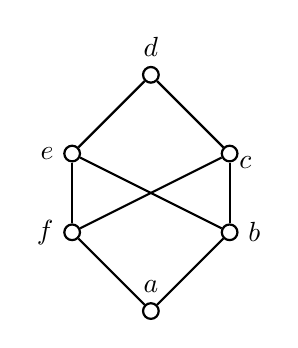
\begin{tikzpicture}
        [nodedecorate/.style={shape=circle,inner sep=2pt,draw,thick},%
        arrowdecorate/.style={-,>=stealth,thick}]
        %% nodes or vertices
        
        \foreach \nodename/\x/\y/\direction/\navigate in { a/3/-3/above/north,
          b/4/-2/right/east, c/4/-1/right/south, d/3/0/above/north, e/2/-1/left/west, f/2/-2/left/west}
        {
          \node (\nodename) at (\x,\y) [nodedecorate] {};
          \node [\direction] at (\nodename.\navigate) {$\nodename$};
        }
        %% edges or lines
        \path
        \foreach \startnode/\endnode/\direction in {a/b/above,
          b/c/below, c/d/left, d/e/below, e/f/below, f/a/below, f/c/left, b/e/right}
        {
          (\startnode) edge[arrowdecorate] node[\direction] {} (\endnode)
        };
      \end{tikzpicture}
    }
    \quad
    \subfigure{
      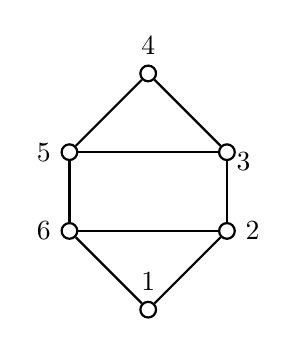
\begin{tikzpicture}
        [nodedecorate/.style={shape=circle,inner sep=2pt,draw,thick},%
        arrowdecorate/.style={-,>=stealth,thick}]
        %% nodes or vertices
        
        \foreach \nodename/\x/\y/\direction/\navigate in { 1/3/-3/above/north,
          2/4/-2/right/east, 3/4/-1/right/south, 4/3/0/above/north, 5/2/-1/left/west, 6/2/-2/left/west}
        {
          \node (\nodename) at (\x,\y) [nodedecorate] {};
          \node [\direction] at (\nodename.\navigate) {$\nodename$};
        }
        %% edges or lines
        \path
        \foreach \startnode/\endnode/\direction in {1/2/above,
          2/3/below, 3/4/left, 4/5/below, 5/6/below, 6/1/below, 6/2/left, 5/3/right}
        {
          (\startnode) edge[arrowdecorate] node[\direction] {} (\endnode)
        };
      \end{tikzpicture}
    }
  }
  \quad
  \subfigure{
    \subfigure{
      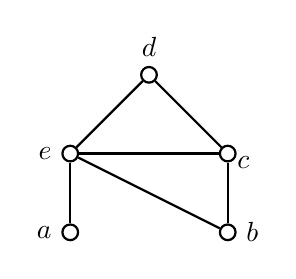
\begin{tikzpicture}
        [nodedecorate/.style={shape=circle,inner sep=2pt,draw,thick},%
        arrowdecorate/.style={-,>=stealth,thick}]
        %% nodes or vertices
        
        \foreach \nodename/\x/\y/\direction/\navigate in { a/2/-2/left/west,
          b/4/-2/right/east, c/4/-1/right/south, d/3/0/above/north, e/2/-1/left/west}
        {
          \node (\nodename) at (\x,\y) [nodedecorate] {};
          \node [\direction] at (\nodename.\navigate) {$\nodename$};
        }
        %% edges or lines
        \path
        \foreach \startnode/\endnode/\direction in {b/c/below, c/d/left, e/a/left, e/b/below, d/e/below, e/c/right}
        {
          (\startnode) edge[arrowdecorate] node[\direction] {} (\endnode)
        };      
      \end{tikzpicture}
    }
    \quad
    \subfigure{
      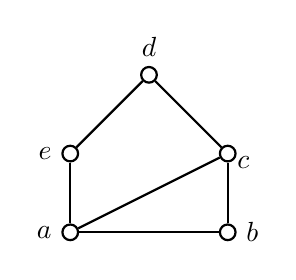
\begin{tikzpicture}
        [nodedecorate/.style={shape=circle,inner sep=2pt,draw,thick},%
        arrowdecorate/.style={-,>=stealth,thick}]
        %% nodes or vertices
        
        \foreach \nodename/\x/\y/\direction/\navigate in { a/2/-2/left/west,
          b/4/-2/right/east, c/4/-1/right/south, d/3/0/above/north, e/2/-1/left/west}
        {
          \node (\nodename) at (\x,\y) [nodedecorate] {};
          \node [\direction] at (\nodename.\navigate) {$\nodename$};
        }
        %% edges or lines
        \path
        \foreach \startnode/\endnode/\direction in {a/b/below, a/c/below, b/c/below, c/d/left, e/a/left, d/e/below}
        {
          (\startnode) edge[arrowdecorate] node[\direction] {} (\endnode)
        };      
      \end{tikzpicture}
    }
  }
  \caption{Изоморфни ли са графите?}
\end{figure}


%%% Local Variables: 
%%% mode: latex
%%% TeX-master: "ds1"
%%% End: 
